\section{Pressions et loi de Boyle-Mariotte}

\begin{frame}{Qu’est-ce que la pression ?}
  \begin{block}{Définition}
    La pression est une \textbf{force exercée perpendiculairement} sur une surface.\\[4pt]
    \[
      P = \frac{F}{S}
    \]
    avec $P$ en bar, $F$ en newton (ou kg) et $S$ en cm\textsuperscript{2}.
  \end{block}

  \begin{itemize}
    \item Unité pratique en plongée : \textbf{bar}.
    \item 1 bar $\approx$ 1 kg/cm\textsuperscript{2}.
  \end{itemize}
\end{frame}

\begin{frame}{Pression atmosphérique}
  \begin{itemize}
    \item La Terre est entourée d’une \textbf{couche d’air} : l’atmosphère.
    \item Le poids de cette atmosphère exerce une pression sur tous les corps.
    \item À la surface de la mer, on considère :
          \[
            P_{\text{atm}} = 1 \text{ bar}
          \]
  \end{itemize}
\end{frame}

\begin{frame}{Pression hydrostatique (relative)}
  \begin{columns}[c]
    \begin{column}{0.62\textwidth}
    \begin{itemize}
      \item Colonne d’eau de 10 m de haut sur 1 cm\textsuperscript{2} :
            \begin{itemize}
              \item Volume = 1 dm\textsuperscript{3} = 1 L $\Rightarrow$ masse $\approx 1$ kg.
              \item $\Rightarrow P = 1$ bar.
            \end{itemize}
      \item \textbf{Règle pratique :} la pression augmente de \textbf{1 bar tous les 10 m}.
      \item À 20 m : $P_{\text{eau}} = 2$ bar, à 30 m : 3 bar, etc.
    \end{itemize}
    \end{column}

    \begin{column}{0.38\textwidth}
      \centering
      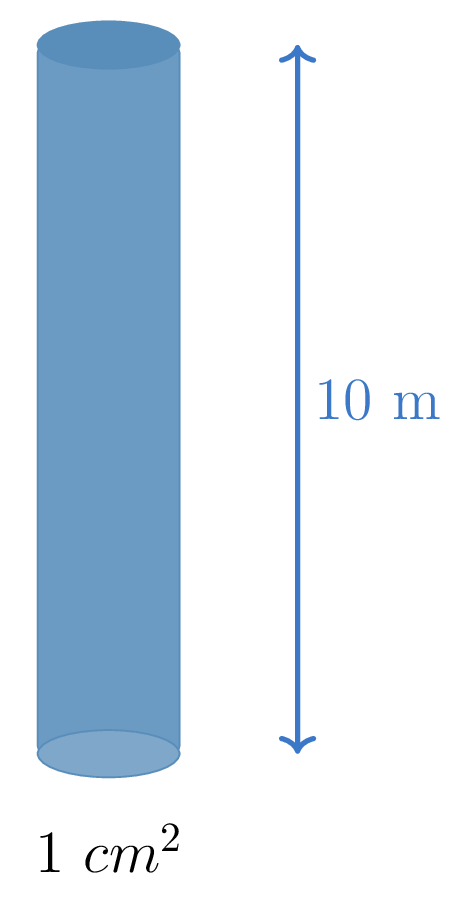
\includegraphics[height=0.6\textheight]{images/colonne_pression}
    \end{column}
  \end{columns}
\end{frame}

\begin{frame}{Pression absolue}
  \begin{block}{Définition}
    \[
      P_{\text{abs}} = P_{\text{atm}} + P_{\text{hydro}}
    \]
  \end{block}

  \begin{itemize}
    \item Surface : $P_{\text{abs}} = 1$ bar.
    \item 10 m : $P_{\text{abs}} = 1 + 1 = 2$ bar.
    \item 20 m : $P_{\text{abs}} = 1 + 2 = 3$ bar.
    \item 30 m : $P_{\text{abs}} = 1 + 3 = 4$ bar.
    \item 40 m : $P_{\text{abs}} = 1 + 4 = 5$ bar.
  \end{itemize}
\end{frame}

\begin{frame}{Loi de Boyle-Mariotte}
  \begin{block}{Énoncé}
    Pour une quantité de gaz donnée à température constante :
    \[
      P \times V = \text{constante} \quad \Rightarrow \quad P_1 V_1 = P_2 V_2
    \]
  \end{block}

  \begin{itemize}
    \item Le corps humain contient :
          \begin{itemize}
            \item des \textbf{solides} (os) et des \textbf{liquides} (sang), \alert{incompressibles},
            \item des \textbf{gaz} (poumons, sinus, oreilles, tube digestif), \alert{compressibles}.
          \end{itemize}
    \item Les volumes d’air \textbf{diminuent à la descente} et \textbf{augmentent à la remontée}.
  \end{itemize}
\end{frame}

\begin{frame}{Exemple simple}
  \begin{columns}[c]
    \begin{column}{0.6\textwidth}
      \begin{itemize}
        \item Ballon d’1 L en surface ($P = 1$ bar).
        \item À 10 m ($P = 2$ bar) :
              \[
                1 \times 1 = 2 \times V_2 \Rightarrow V_2 = 0{,}5 \text{ L}
              \]
        \item À 20 m ($P = 3$ bar) :
              \[
                1 \times 1 = 3 \times V_3 \Rightarrow V_3 \approx 0{,}33 \text{ L}
              \]
      \end{itemize}
    \end{column}
    \begin{column}{0.4\textwidth}
      \centering
      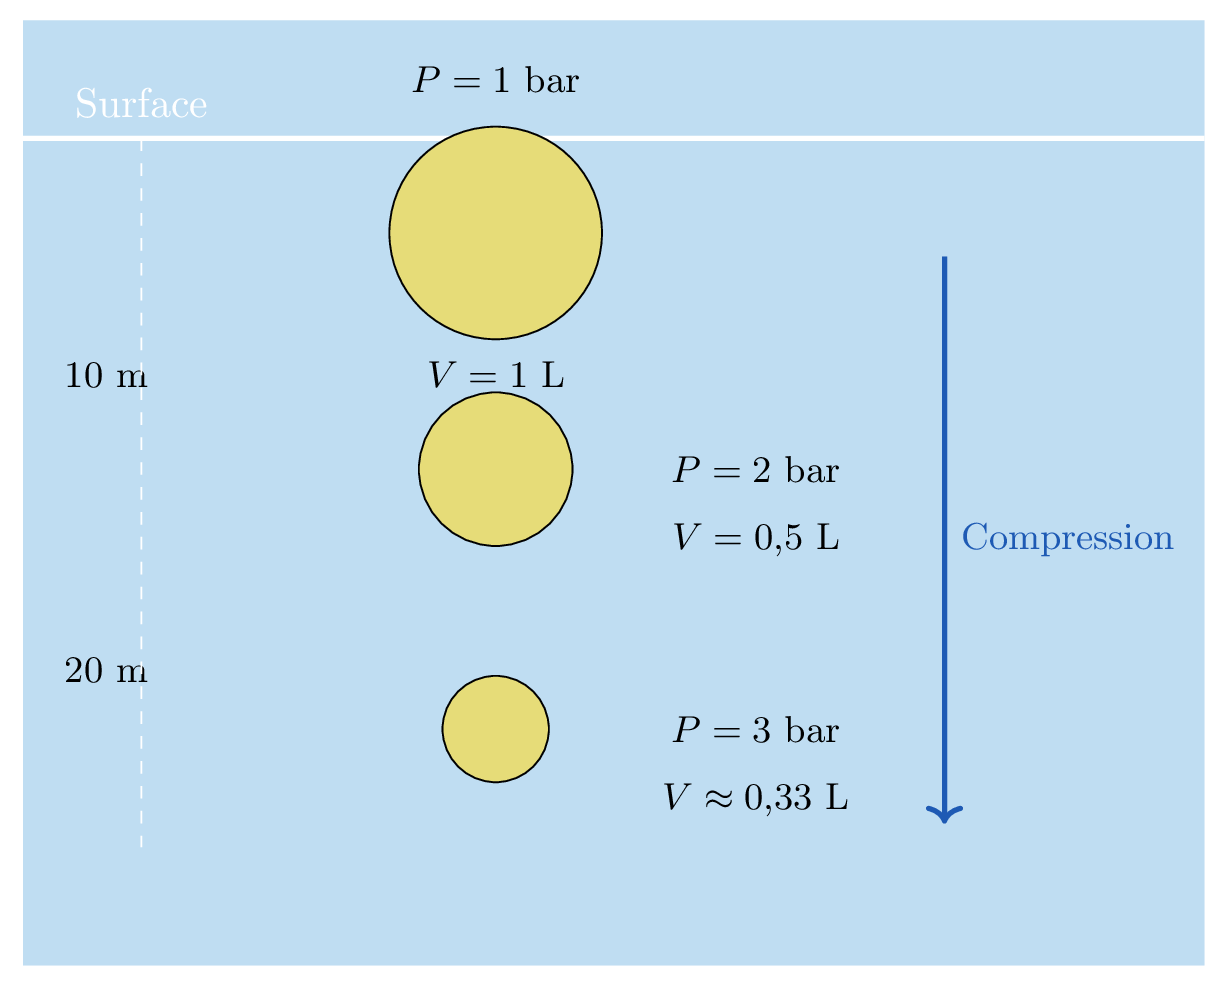
\includegraphics[height=0.6\textheight]{images/ballons_compression}
    \end{column}
  \end{columns}
\end{frame}

\begin{frame}{Conséquences pour le plongeur}

  \begin{block}{À retenir (essentiel)}
    \begin{itemize}
      \item Les espaces remplis d’air se \textbf{compressent} à la descente
            et se \textbf{dilatent} à la remontée.
      \item \alert{Ne jamais bloquer sa respiration à la remontée.}
    \end{itemize}
  \end{block}

  \vspace{0.15cm}

  \begin{block}{Conséquences pratiques}
    \begin{itemize}
      \item À la remontée, \textbf{expirer en continu}, surtout entre
            \textbf{0 et 10 m} (la pression y \textbf{double}).
      \item \textbf{La consommation d’air augmente avec la profondeur}
            (gaz plus dense, pression plus élevée).
      \item \alert{Ne jamais donner de l’air à un plongeur en apnée}
            $\rightarrow$ risque majeur de \textbf{surpression pulmonaire}.
      \item Ces variations expliquent les \textbf{accidents barotraumatiques}
            (oreilles, sinus, masque, dents, poumons).
    \end{itemize}
  \end{block}

\end{frame}
